% Name: Lattice paths
% Description: One of the 35 shortest paths along a 4 by 3 grid from the bottom-left corner to the top-right, each a choice of which 3 of its 7 steps go up.
% Tags: lattice paths, binomial coefficient, grid, combinatorics

\usepackage{amsmath}
\usetikzlibrary{arrows.meta}

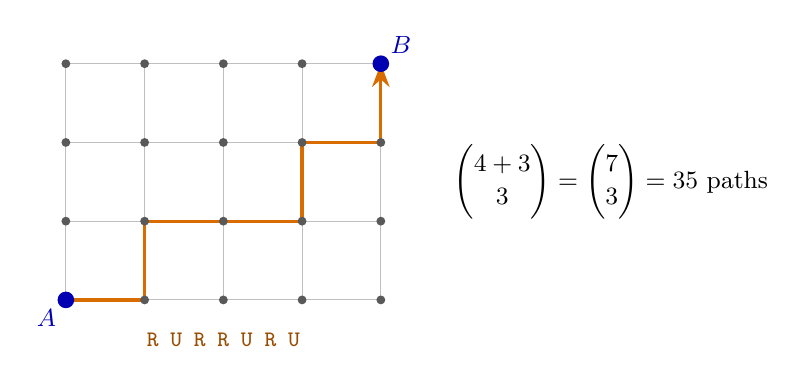
\begin{tikzpicture}[>={Stealth}, every node/.style={font=\small}]
  \draw[gray!50, thin] (0,0) grid (4,3);
  % Steps R, U, R, R, U, R, U: right 4 times and up 3 times
  \draw[->, very thick, orange!85!black, line join=round] (0,0) -- (1,0) -- (1,1) -- (3,1) -- (3,2) -- (4,2) -- (4,3);
  \foreach \x in {0,...,4} \foreach \y in {0,...,3} \fill[gray!70!black] (\x,\y) circle (1.6pt);
  \fill[blue!70!black] (0,0) circle (3pt) node[below left] {$A$};
  \fill[blue!70!black] (4,3) circle (3pt) node[above right] {$B$};
  \node[below=1mm, font=\footnotesize\ttfamily, orange!60!black] at (2,-0.2) {R U R R U R U};
  \node[anchor=west] at (4.8,1.5) {$\dbinom{4+3}{3} = \dbinom{7}{3} = 35$ paths};
\end{tikzpicture}
